\chapter{Operational Transconductance Amplifier}

\section{Design and Implementaion}

The first stage of the design is the Operational Transconductance Amplifier. This stage uses bipolar power supply of 2.5V and -2.5V. 

\subsubsection{Commercial OTA}
OPA860 by Texas Instruments is one of the most popular commercial OTA in the market. The design document(citation) of OPA860 compares OTA to a 3 terminal transistor - a high impedance input(base), low impedance inout(emitter) and a current output(collector). OTA is therefore bipolar and self-biased. Being self-biased simplifies the design process and reduces component count. The overview of the OTA is as shown in Figure.\ref{fig:OPA}. The transconductance of the OTA can be adjusted using an external resistor, allowing bandwidth, quiscent current and gain trade-offs to be optimized. Reducing or increasing the size of the OTA controls the bandwidth, AC behavior and transconductance. With a fixed external resistor, the quiscent current increases with increase in temperature. The variation of the current with temperature holds the transconductance of the OTA relatively constant with temperature.

\begin{figure} [H]
\centering
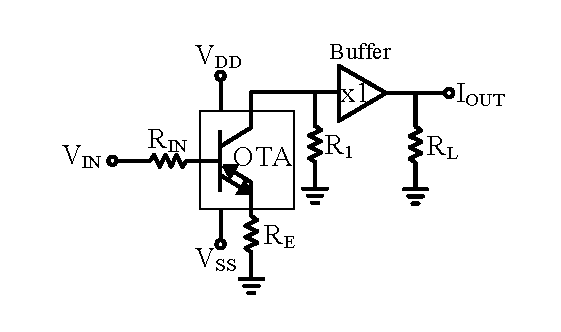
\includegraphics[scale=1]{Figures/Misc/PDFs/OPA.pdf}
\caption{Overview of Commercial OTA OPA860}
\label{fig:OPA}
\end{figure}

The commercial OTA in review, can operate in 2 modes - Voltage mode and Current mode. In voltage mode, it can operate in 3 states - common emitter, common base and common collector. In current mode, it is useful for analog communication such as current amplifier, current differentiator, current integrator and current summer. The output offset voltage is usually very close to zero for an OTA.

Having stated all these facts, this commercial OTA is an amplifier based on BJTs. Considering the high power dissipation and high input current noise of a BJT based amplifier, it is not suitable for our system. However, the concept of having an OTA and an output buffer is something that can be pondered upon.

\subsubsection{Self-Cascode OTA}
An intruiging concept of Self-Cascode can be used to achieve very high gain for a low supply voltage. A high gain 2-stage self cascode OTA for a 1V supply was researched as part of (citation). A self-cascode MOSFET (SCMOS) has a similar geometrical structure to a regular MOSFET. But still, the transconductance, and the output resistance of an SCMOS are much better than its conventional counterpart. A regular channel requires a long channel for high gain and a short channel for high speed. With the same channel length of a regular MOS, an SCMOS will provide a much higher gain without compromising the speed. 
An SCMOS is formed where a regular MOSFET will be replaced by two transistors whose gates are tied together, as shown in Figure.\ref{fig:SCMOS}. The two transistors have same widths. The operating regions of $M_1$ and $M_2$ depend upon the common gate voltage of the SCMOS. If $V_g$ is greater than $V_{th}$ of both the MOSFETs, then $M_1$ and $M_2$ operate in linear and saturation region respectively. With a bulk bias, the threshold voltage of the drain transistor ($M_2$) decreases. This increases the $V_{ds}$ of $M_1$, resulting in moving of its operating point from linear to edge of saturation, i.e., moderate inversion. And this is where the gain is high. Suppose both transistors are operating in saturation, the maximum output resistance can be achived but the voltage swing is considerably reduced.

\begin{figure} [H]
\centering
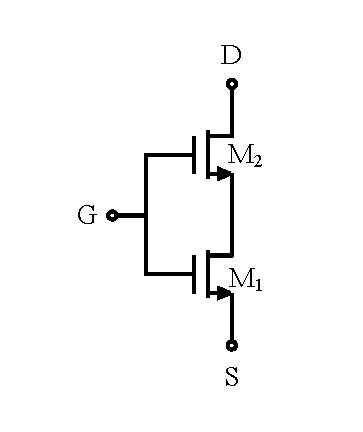
\includegraphics[scale=1]{Figures/Misc/PDFs/SCMOS.pdf}
\caption{Schematic of a Self-Cascode MOSFET}
\label{fig:SCMOS}
\end{figure}

In the context of an OTA, consider a conventional OTA with their regular MOSFETs replaced by SCMOS. To improve the gain of the OTA, positive feedback is created by cross coupling the bulk terminals of the input stage load transistors. Smaller channel length CMOS requires scaling down of power supply to maintain reliability of the circuit. A dual function gate MOSFET with a focus on increasing output resistance and transconductance is equivalent to a self cascode structure. A floating gate MOSFET is another alternative to the conventional techniques used to enhance DC gain. But, both these techniques require complicated fabrication steps. On the other hand, a current shunt technique can be applied to a self-cascode OTA to increase its gain. But this has reduced phase margin and requires compensation circuit even for a single stage.

A self-cascode OTA is very hekpful in achieving a high gain for low power supplies. But give the nature of our system, and the fact that the OTA to be designed as part of this system is to be an open loop amplifier, a very high gain is something that is suitable for the system in order to avoid saturation at the output as the headroom for output transistors would be very less. Another possible drawback is that the self-cascode OTA exhibits a slew rate that is lesser than the conventional OTA because the output current is low. But in case our system had to work in a closed loop, then this concept of self-cascode would have been a better fit.

\subsubsection{2-stage Feed Forward Miller Compensation OTA}

The system level diagram of a feed-forward Miller compensated OTA is shown in Figure.\ref{fig:FFMCO}. The $g_{m1}$ and $g_{m2}$ are input and output stage of the OTA and $g_{mf}$ is the feed-forward path from input to output node. The implementation is based on feed-forward technique proposed in (citation). There is no concept of pole spiltting. The location of poles is mainly dependent on the internal node impedance and parasitic capacitance. It is difficult to estimate the parasitic capacitances and it makes the design complex. Therefore the dominant and non-dominant pole locations will change when the OTA is configured in a closed loop. But using Miller compensation, the poles can be placed at desired locations.

\begin{figure} [H]
\centering
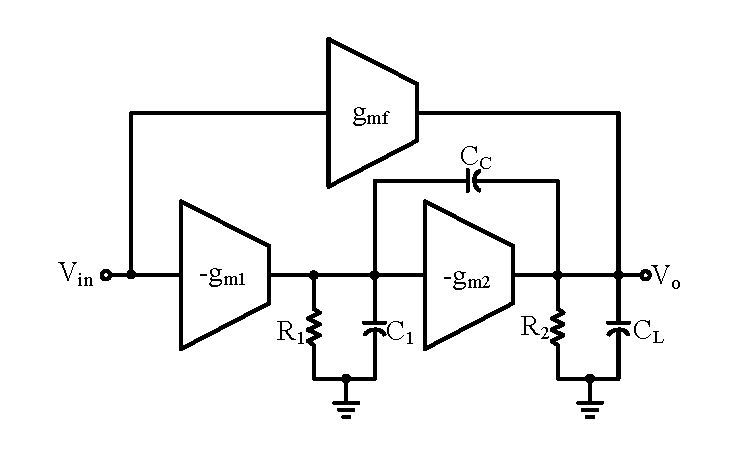
\includegraphics[scale=1]{Figures/Misc/PDFs/FFMCO.pdf}
\caption{Block Diagram of Feed Forward Miller Compensation OTA}
\label{fig:FFMCO}
\end{figure}

This topology of OTA is considered to consume less power than the conventional Miller compensation OTA. Feed forward compensation technique gives wider bandwidth as compared to the Miller OTA and is much more easier to stabilize.  However the overall bandwidth is lesser than what a conventional current mirror based OTA can provide. Current replicating branch with scaled down transistors can be used to implement a push-pull output stage that gives the maximum output current several times higher than that of bias current. Cascoding and gain boosting are conventional techniques for gain enhancement. But for low voltage designs, these techniques are not suitable due to limited head room. Cascading multiple gain stages is another alternative for the gain enhancement. But in a closed loop, the amplifier becomes unstable due to high impedance nodes at each stage, which produces negative phase shift and degrades the overall phase margin. To overcome this, the multi-stage amplifier needs a compensation circuit to achieve a minimum phase margin for stability.

The results of this topology were interesting and encouraging. But that fact that needs multiple stages and compensation circuitry just for a OTA without a buffer, makes it complex in spite of the encouraging remedies. So weighing the pros and cons of the topology and comparing it with other OTAs in review, this topology was deemed to be a bit too much for our requirements and question of feasibility comes into picture.

\subsubsection{A robust Feed Forward scheme without Miller capacitance}

This scheme uses a positive phase shift of left hand plane (LHP) zeros caused by the feedforward path to cancel the negative phase shift of poles to attain good phase margin. The two-stage path increases the low frequency gain further  while the feed forward single stage amplifier makes the circuit faster. The amplifier bandwidth is not compromised by the absence of the traditional pole-splitting effect of Miller compensation capacitor, resulting in a high gain wide-band amplifier.

\begin{figure} [H]
\centering
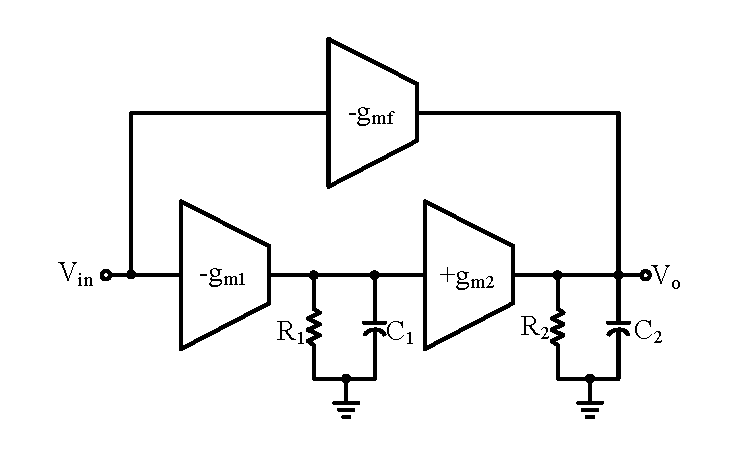
\includegraphics[scale=1]{Figures/Misc/PDFs/FFNMCO.pdf}
\caption{Block Diagram of Feed Forward OTA without Miller Capacitor}
\label{fig:FFMNCO}
\end{figure}

Amplifiers with high-gain generally use multi-stage designs. And trasistors with long channgel length are chosen and biased at low current levels. Amplifiers with high-bandwidth use single-stage designs with short channel length transistors biased at high current levels. In a Miller compensated amplifier, due to the Miller effect, the dominant pole is pushed towards lower frequencies, resulting in lower bandwidth. Along with this, the phase response is degraded with a RHP zero. A nulling resistor is used to cancel the effect of this RHP zero. The pole-zero pair is created at high frequencies to acoid the slow settling components associated with pole-zero cancellation at low frequencies. 

This scheme results in an amplifier with high gain and fast respsone. Bandwidth improvement is due to the fact that poles are not split. There could be substantial reduction in the area and power as there is no Miller compensation capacitor. As part of the circuit realization, the second andd feed-forward stage should not have any dominant pole before overal frequency for gain bandwidth. Pole-zero cancellation should occur at high frequencies for best settling time performance. The first stage in this scheme is usually designed to have a high gain and a small load capacitance. The second and feedforward stages should be optimized for high bandwidth and medium gain performance.

This topology offers several advantages over the other topologies reviewed during the design phase. Some aspects to be careful about are - the feed-forward stage has to be optimized to make sure the pole-zero cancellation occurs at high frequency otherwise there is a possibility of having an unstable system. Another drawback as in the previous case is the complexity of the circuit given that this scheme was initially intended to work for a single input design. Having two different pairs to transistors that need biasing at its gate terminals along with the complexity of the design, makes the programmability of the circuit a mystery. And since that is an integral part of our specification, this scheme might not be entirely suitable for our design despite offering more advantages than disadvantages.

\subsubsection{Super Class AB OTA}
The schematic of a Super Class AB OTA based on a Cascode Voltage Flipped Follower is as shown in Figure.\ref{fig:OTA_Class_AB}. It uses a Class-AB differential pair to boost the bias current by a factor of $k_1$. Typical values of $k_1$ range from 30 to 60 depending on the implementation of the Class-AB differential pair and supply voltages. An additional current boosting by a factor of $k_2$ is obtained in the output branches. The typical values of $k_2$ range from 3-8. Using cascode transistors maximum output current and subsequently the CE values are reduced. But lack of cascode transistors results in very low open loop gain. Therefore, a simple power efficient technique is used that allows the use of cascode transistors in order to achieve even higher open loop gain and gain bandwidth by maintaining a large CE value. This is done with the help of dynamically biasing the cascode transistors using RC networks (indicated in purple in the figure). The capacitor $C_{bat}$ acts as a floating battery for dynamic operations that transfers variations in the gate voltages of mirror transistors to the gate of the cascode transistors. This increases the $V_{DS}$ of the mirror transistors allowing high output currents. Cascode Voltage Flipped Follower (indicated in red in the figure) is charaterized by high input swing and can operate over a wide range of supply voltages. It uses local shunt feedback to provide nodes A and B with very low impedance.

\begin{figure} [H]
\centering
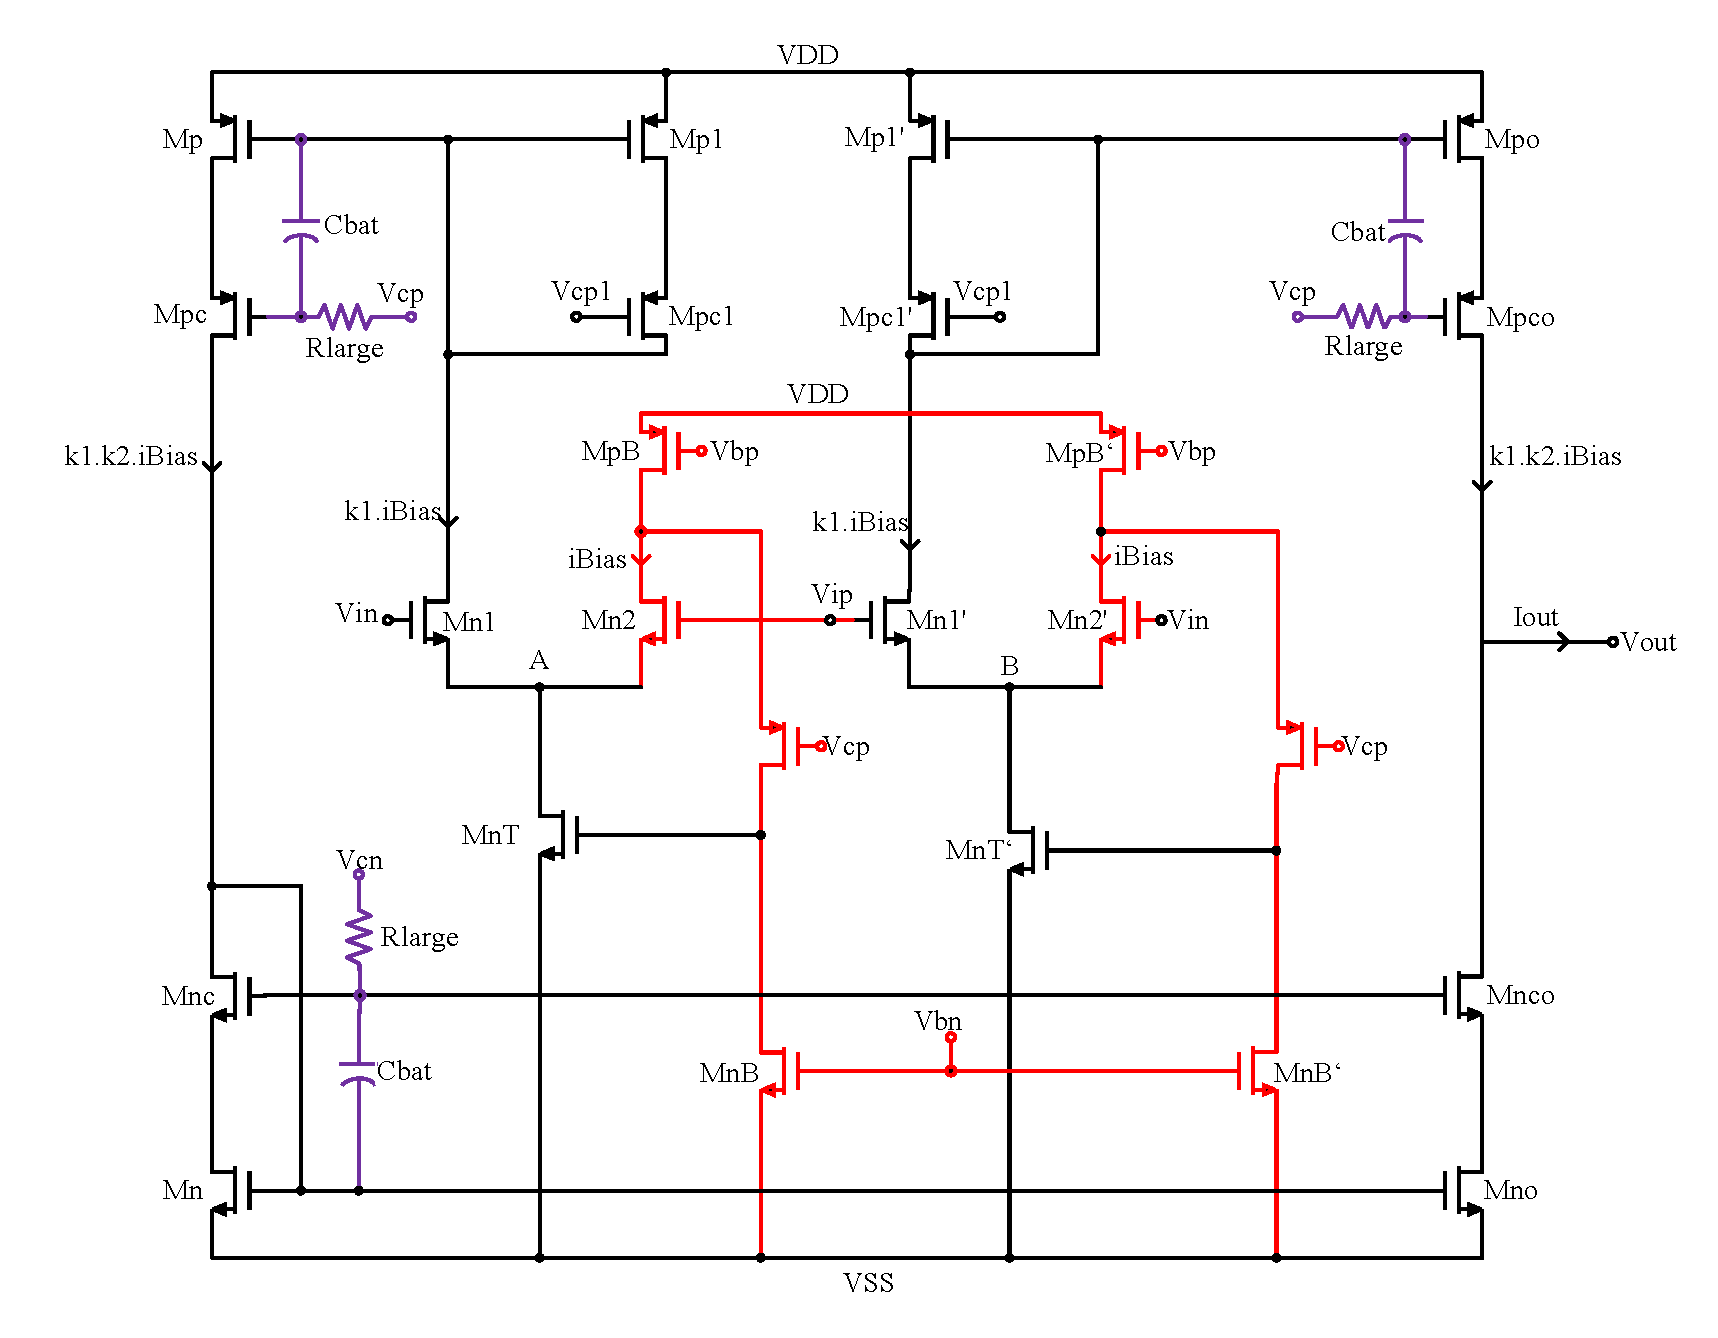
\includegraphics[scale=0.65]{Figures/Schematics/OTA_Class_AB.pdf}
\caption{Super Class-AB OTA with a Cascode Voltage Flipped Follower}
\label{fig:OTA_Class_AB}
\end{figure}

Taking into account the complexity, output current requirements and load requirements, this design will not be considered further as part of this research work. The reason being - a high current output of this Class AB OTA would give rise to another output buffer. And the capacitors needed to consume such a high current would be in the order of several pico Farads. Having such a big capacitor inside an IC is not recommended. Also, considering how complex CMOS Current Feedback Amplifiers are, it is wise to stick to a simpler design that does the same work but with some minor trade-offs.

\subsubsection{Conventional OTA}
Two separate designs - OTA with PMOS Differential pair and OTA with NMOS Differential pair were deisgned and simulated in Cadence to get a good understanding of the circuit parameters and how the differential pair impact them. 

Generally, amplifiers with PMOS transistors used as differential input offer high linearity, low flicker (1/f) noise. A possible reason to choose PMOS transistors as a differential pair comes from the necessity to reduce the influence of the substrate noise. The two transistors are in an N-well and the well is connected to the supply voltage that any substrate interference coupled via the parasitic capacitance to substrate is decoupled to the VDD line. P-channels typically have less flicker noise (1/f noise) caused by the carriers randomly enterring and leaving traps introduced by defects near the semiconductor surface. Since the majority charge carriers are holes in PMOS, there are less potential to be trapped in surface states.

Having stated all these facts, NMOS input transistors would be better in terms of transconductance gain, and hence thermal noise and the bandwidth of the amplifier. An important fact considered in the selection of the type of differential pair is that the OTA in this system is being used in an open loop. This means that the gain of the OTA has to be limited in order to avoid saturation at the crests and troughs at the output of the OTA.

PMOS transistors exhibit their low noise behaviour due to the fact that PMOS transistors are usually bigger (higher W/L ratio) than an NMOS pair. Since we need a small open loop gain, we cannot afford to have big transistors at the input that cause the output to saturate. Along with this, it was also seen that, the range of bias currents needed to obtain a similar range of voltage swing was much wider in case of PMOS than NMOS. Since this indirectly results in a high power dissipation in the 1st stage itself, it was concluded to use the NMOS based design as part of this Thesis work.

\subsection{Schematic}

Figure.\ref{fig:OTA_Schematic} shows the schematic of the OTA used as part of this Thesis. As mentioned above, the differential amplifier is formed by the NMOS pair. The bias current $I_{bias}$ to the differential pair is provided by the current mirror formed by $M_{nB1}$ and $M_{nB2}$ which is in turn controlled by the PMOS transistor $M_9$ whose gate voltage $V_{bias}$ is the programmable variable of the OTA and the entire system. This bias voltage is inversely proportional to the bias current flowing through each branch of the OTA.

\begin{figure} [H]
\centering
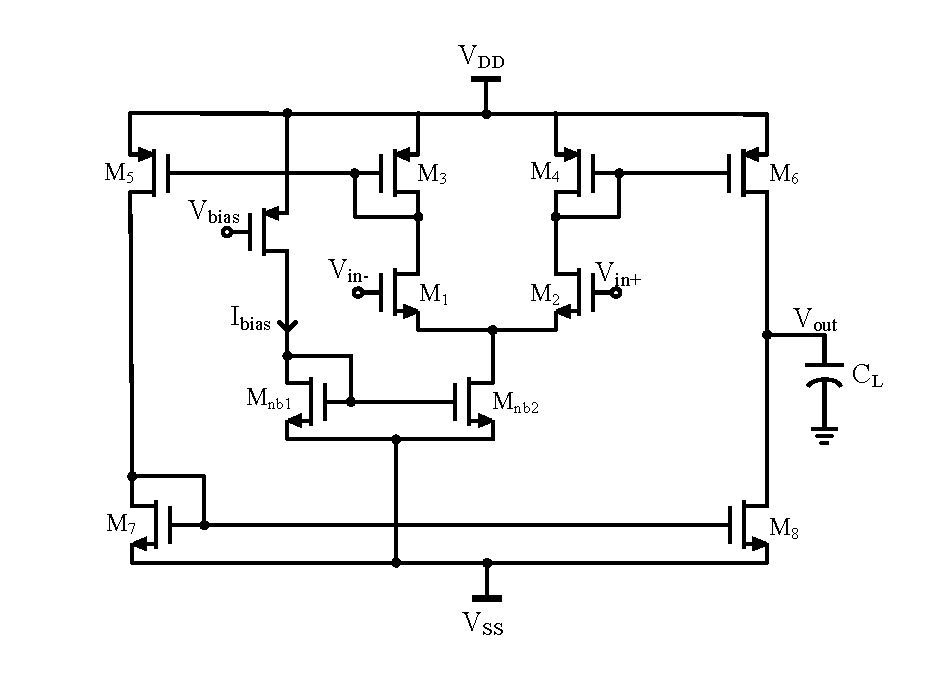
\includegraphics[scale=1]{Figures/Schematics/OTA_NMOS_Vbias.pdf}
\caption{Schematic of the OTA Designed}
\label{fig:OTA_Schematic}
\end{figure}

\begin{table} [H]
\centering
\begin{tabular}{@{}cccc@{}}
\toprule
Transistor			& Width				& Length			& Multiplier \\ \midrule
M1					& 8u				& 500n				& 5			\\
M2					& 8u				& 500n				& 5			\\
M3					& 35u				& 500n				& 1			\\
M4					& 35u				& 500n				& 1			\\
M5					& 28u				& 500n				& 3			\\
M6					& 35u				& 500n				& 3			\\
M7					& 35u				& 500n				& 18		\\
M8					& 33u				& 500n				& 18		\\
M9					& 10u				& 500n				& 4			\\
MnB1				& 20u				& 500n				& 8			\\
MnB2				& 20u				& 500n				& 8			\\
\bottomrule
\end{tabular}
\caption{Dimensions of the Transistors of the designed OTA}
\label{tab:OTA_dimensions}
\end{table}


From the Table.\ref{tab:OTA_dimensions}, it can be seen that the current mirror gain for the current mirrors formed by $M_{3}$, $M_{5}$ and $M_{4}$, $M_{6}$ is 3. It can also be noted that the transistors $M_{5}$ and $M_{8}$ are not symmetric with respect to their counterparts. This is designed so to make sure the DC bias point at the output of the OTA is close to 0V, which is the mid point of $V_{DD}$ and $V_{SS}$. Changing the bias current of an amplifier, will automatically change the DC bias point at its output. Since we are using the OTA as a programmable block, it is important to have an output which is symmetric over 0. Even though it is not entirely possible, making these two transistors a little assymetric or uneven would close the gap between the bias points for highest and lowest bias currents.

\section{Test Setup}
In the following subsections, let us look at how this $V_{bias}$ affects various paramters of the OTA by performing DC, AC, Transient and Noise Analyses.

\begin{figure} [H]
\centering
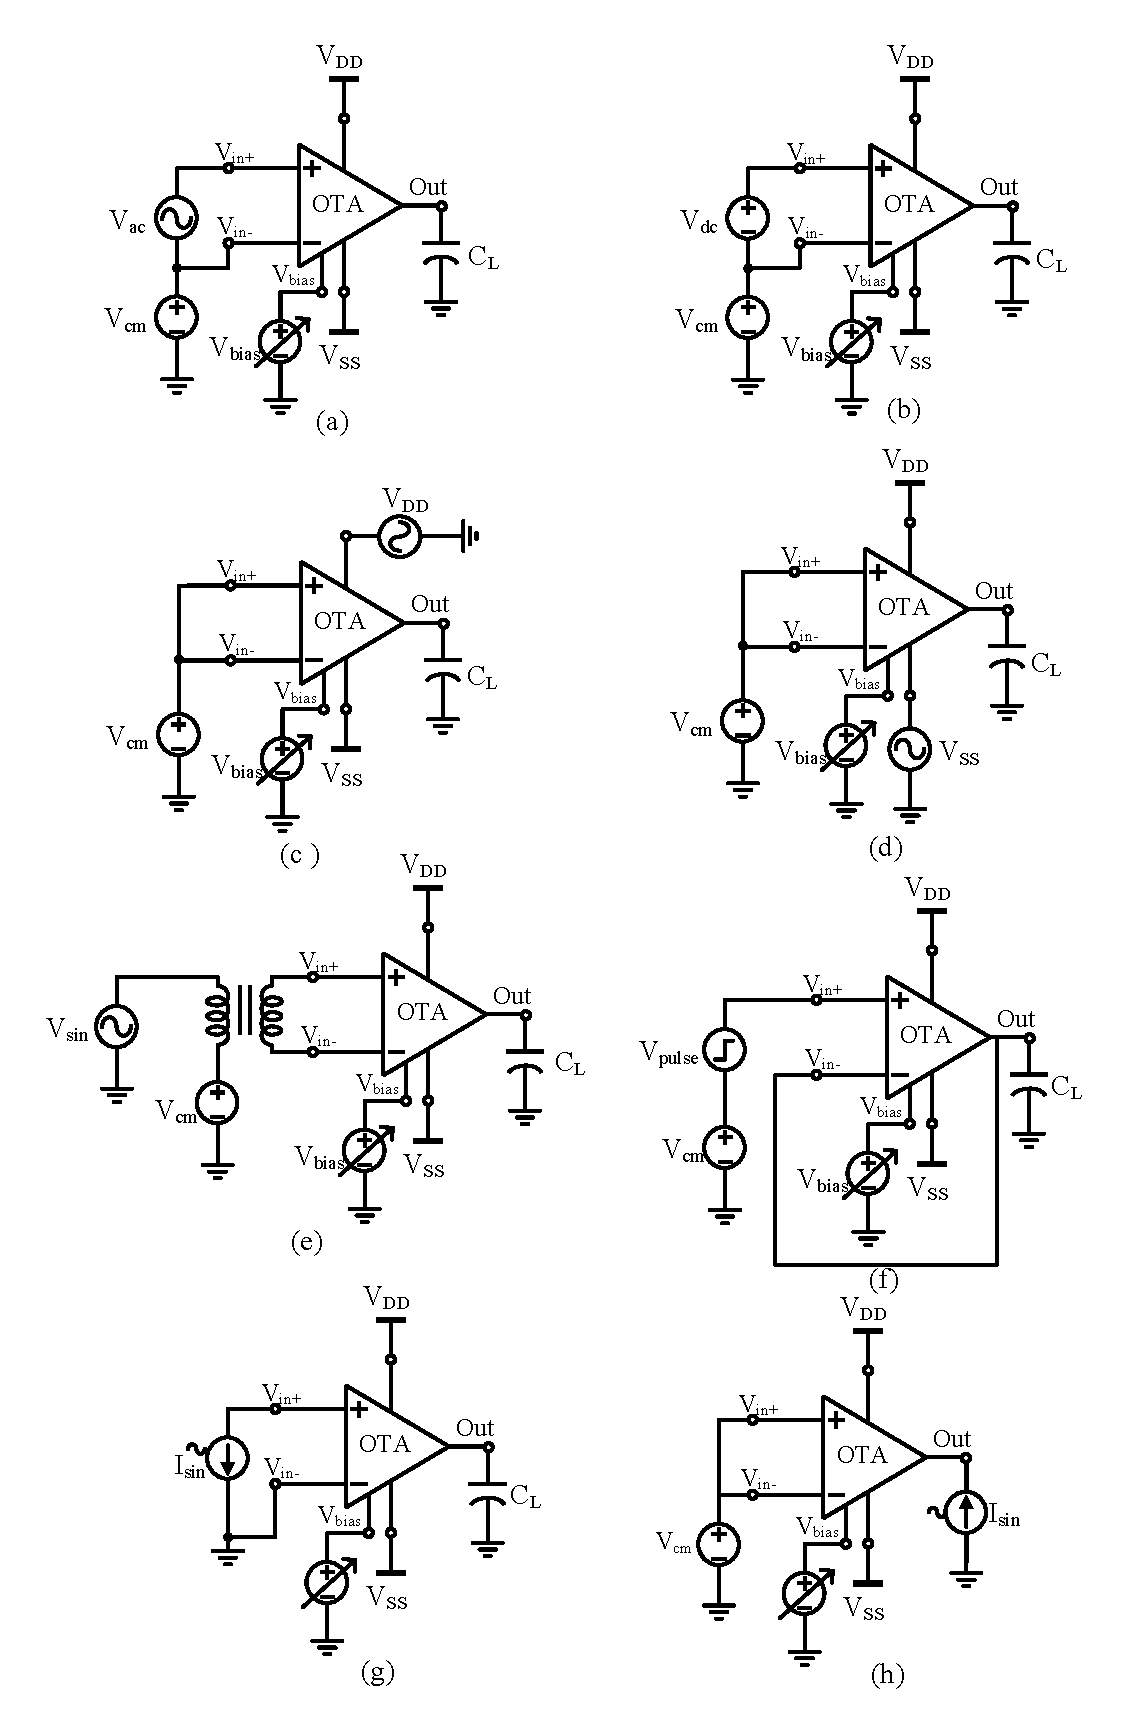
\includegraphics[scale=0.8]{Figures/Test_Benches/OTA_TB.pdf}
\caption{Test bench setup for OTA}
\label{fig:OTA_TB_ACDC}
\end{figure}

\subsection{DC Analysis}

$V_{DD}$ = 2.5V; $V_{SS}$ = -2.5V; $V_{cm}$ = 1.95V; $V_{bias}$ = 150mV to 700mV;  $V_{ac}$ = 1V; $C_{L}$ = 50fF.


\begin{table} [H]
\centering
\begin{tabular}{@{}cccccccc@{}}
\toprule
Vbias (mV)					& 150		& 200			& 300			& 400			& 500			& 600			& 700 \\ \midrule
Output DC Bias (mV)			& 13.68		& -16.43		& -78.96		& -144.6		& -213.3		& -285.2		& -360.3 \\
\bottomrule
\end{tabular}
\caption{Output DC Bias Point of the OTA}
\label{tab:OTA_DC_Bias}
\end{table}

The output DC bias points for various values of $V_{bias}$ is tabulated in Table\ref{tab:OTA_DC_Bias}. The DC voltage at the output decreases with the increase in bias voltage or decrease in bias current.

\subsection{AC Analysis}
\subsubsection{Gain, Bandwidth and Phase Margin}
$V_{DD}$ = 2.5V; $V_{SS}$ = -2.5V; $V_{cm}$ = 1.95V; $V_{bias}$ = 150mV to 700mV;  $V_{ac}$ = 1V; $C_{L}$ = 50fF.

The same parameters hold good for AC analysis as well. Here, the value of $V_{ac}$ becomes significant. The value of the open loop gain is given by the ratio of output voltage to input voltage.

Gain = $\frac{V_{out}}{V_{in}}$\\
Gain in dB = $20 log_{10}\frac{V_{out}}{V_{in}}$

Figure\ref{fig:OTA_Gain} shows the semilog plot of Gain for maximum and minimum $V_{bias}$. The plots for the other values of $V_{bias}$ are not shown here as that would make the plot less legible for understanding and more so because those plots would be in between the plots already shown.

\begin{figure} [H]
\centering
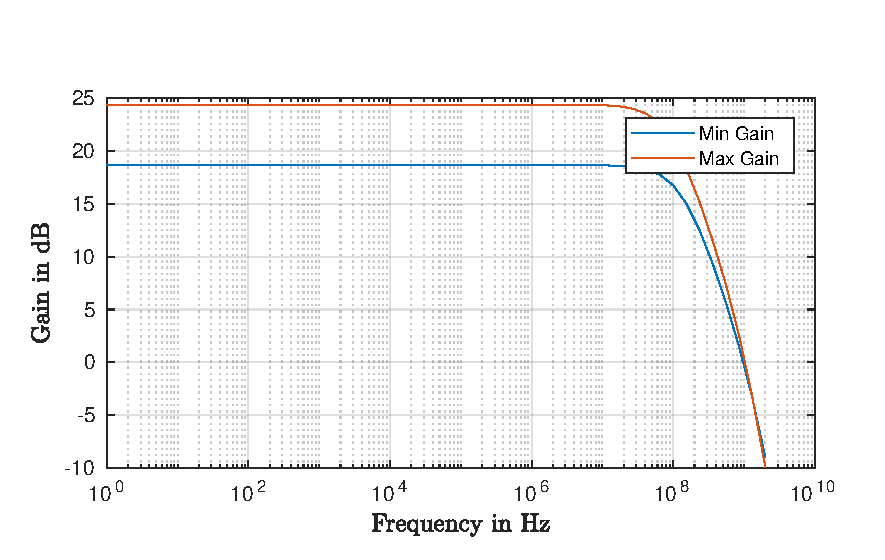
\includegraphics[scale=1]{Figures/Plots/OTA_Gain.pdf}
\caption{OTA Plot of Gain vs Frequency for different Vbias}
\label{fig:OTA_Gain}
\end{figure}

The variation of open loop gain of the OTA, its bandwidth and the phase margin with respect to $V_{bias}$ is tabulated in Table.\ref{tab:OTA_gain_bw_pm}. The bandwidth is kept at a high value in order to make sure that the dominant poles of the first and second stages are sufficiently far from each other so as to obtain a stable system for operation. The maximum open loop gain for this system is 23.7dB. Any value beyond this will cause the amplifier to saturate at the crests and troughs of the output voltage.

\begin{table} [H]
\centering
\begin{tabular}{@{}cccccccc@{}}
\toprule
Vbias (mV)					& 150		& 200		& 300		& 400		& 500		& 600		& 700 \\ \midrule
Open Loop Gain (dB)			& 18.64		& 19.46		& 20.9		& 22.05		& 22.96		& 23.7		& 24.35 \\
Phase Margin (degrees)		& 63.3		& 60.63		& 55.96		& 52.42		& 49.91		& 48.12		& 46.72 \\
Bandwidth (MHz)				& 135		& 130.7		& 122.2		& 113.7		& 105		& 96.63		& 89.19 \\
\bottomrule
\label{tab:OTA_gain_bw_pm}
\end{tabular}
\caption{Open Loop Gain, Phase Margin and Bandwidth of the OTA}
\end{table}

\begin{figure} [H]
\centering
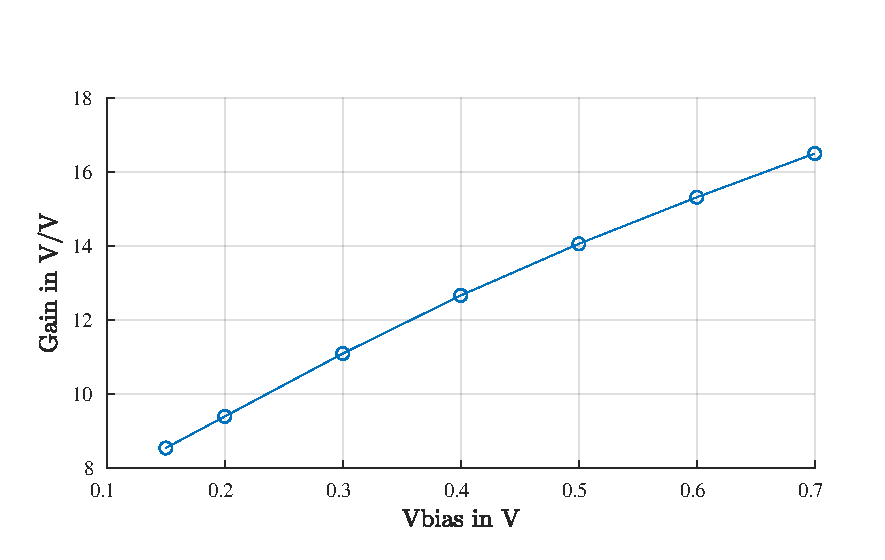
\includegraphics[scale=1]{Figures/Plots/OTA_Gain_Abs.pdf}
\caption{OTA Plot of Gain vs Vbias}
\label{fig:OTA_gain_abs}
\end{figure}

On the same lines, the variation of absolute value of gain with respect to different values of $V_{bias}$ is seen in Figure\ref{fig:OTA_gain_abs} tabulated in Table.\ref{tab:OTA_gain_abs}. The reason to choose the values of $V_{bias}$ are evident from this table and that is because it provides us a gain in the ratio of almost 1:2 for those values of $V_{bias}$. As seen from the table of specifications that we need a transconductance in the ratio of 1:1.8 or something close to that.

\begin{table} [H]
\centering
\begin{tabular}{@{}cccccccc@{}}
\toprule
Vbias (mV)					& 150			& 200			& 300			& 400			& 500			& 600			& 700 \\ \midrule
DC Gain (V/V)			& 8.548		& 9.4		& 11.1		& 12.67		& 14.06		& 15.31		& 16.49 \\
\bottomrule
\end{tabular}
\caption{Absolute values of DC Gain of the OTA}
\label{tab:OTA_gain_abs}
\end{table}

\subsubsection{PSRR}

$ PSRR = \frac{\Delta I_{out}}{\Delta V_{DD}}$

$V_{DD}$ = 2.5V; $AC Magnitude of V_{DD}$ = 1V; $V_{SS}$ = -2.5V; $V_{cm}$ = 1.95V; $V_{bias}$ = 150mV to 700mV; $C_{L}$ = 50fF.

$V_{DD}$ = 2.5V; $V_{SS}$ = -2.5V; $AC Magnitude of V_{SS}$ = 1V; $V_{cm}$ = 1.95V; $V_{bias}$ = 150mV to 700mV; $C_{L}$ = 50fF.

The test bench to measure the PSRR of the OTA is as shown in the Figure.(c). The one on the left is used to measure PSRR for a change in $V_{DD}$. And similarly, the one on the right side is used to measure PSRR for a change in $V_{SS}$.

The variation of PSRR with respect to $V_{bias}$ is tabulated in Table.\ref{tab:OTA_PSRR}. The PSRR is fairly low in the range of nA/V and increases only slightly with increase in $V_{bias}$.

\begin{table} [H]
\centering
\begin{tabular}{@{}cccccccc@{}}
\toprule
Vbias (mV)					& 150			& 200			& 300			& 400			& 500			& 600			& 700 \\ \midrule
PSRR (VDD Supply) (nA/V)			& 234.6		& 236.9		& 241.6		& 246.7 	& 252.2		& 258		& 264.3 \\
PSRR (VSS Supply) (nA/V)			& 254.5		& 256.5		& 260.4		& 264.2		& 267.9		& 271.5		& 274.9 \\
\bottomrule
\end{tabular}
\caption{Power Supply Rejection Ratio of the OTA}
\label{tab:OTA_PSRR}
\end{table}

\subsubsection{Input Impedance}
OTAs generally exhibit a very high input impedance. And to measure this parameter, an AC current source with a magnitude of 1A is connected to the non-inverting terminal of the OTA. And the input impedance is given by the ratio of the AC voltage to the AC current at the input of the OTA. Since the current at the input is 1A, the magnitude of the input voltage will be the value of the input impedance in Ohms at that particular frequency. Since the OTA operation is carried out at 1MHz, the voltage at 1MHz is considered to obtain the value of Input Impedance. Figure.(g) shows the test bench to measure the input impedance.

$V_{DD}$ = 2.5V; $V_{SS}$ = -2.5V; $V_{bias}$ = 150mV to 700mV; $C_{L}$ = 50fF; $I_{sin} magnitude$ = 1A. 

The variation of input impedance with respect to $V_{bias}$ is tabulated in Table.\ref{tab:OTA_ZIN}. The variation is quite small and it increases slightly with an increase in bias voltage and is in the order of Mega Ohms.

\begin{table} [H]
\centering
\begin{tabular}{@{}cccccccc@{}}
\toprule
Vbias (mV)					& 150		& 200			& 300			& 400			& 500			& 600			& 700 \\ \midrule
Input Impedance (M$\Omega$)			& 3.38		& 3.388		& 3.403		& 3.419		& 3.434		& 3.45		& 3.467 \\
\bottomrule
\end{tabular}
\caption{Input Impedance of the OTA}
\label{tab:OTA_ZIN}
\end{table}

\subsubsection{Output Impedance}

In a concept similar to measuring the input impedance, the output impedance too, is measured with a help of a current source with unity magnitude at the output instead of a Capacitive load. The differential inputs are connected in a common mode configutation. The test bench to measure the output impedance of the OTA is as shown in Figure(h).

$V_{DD}$ = 2.5V; $V_{SS}$ = -2.5V; $V_{cm}$ = 1.95V $V_{bias}$ = 150mV to 700mV; $I_{sin} magnitude$ = 1A. 
 
As discussed in the theory chapter, OTAs generally have high output impedance. And its variation with respect to $V_{bias}$ is tabulated in the Table.\ref{tab:OTA_ZOUT}
\begin{table} [H]
\centering
\begin{tabular}{@{}cccccccc@{}}
\toprule
Vbias (mV)					& 150		& 200			& 300			& 400			& 500			& 600			& 700 \\ \midrule
Output Impedance (k$\Omega$)			& 1.262		& 1.3		& 1.382		& 1.473		& 1.577		& 1.697		& 1.837 \\
\bottomrule
\end{tabular}
\caption{Output Impedance of the OTA}
\label{tab:OTA_ZOUT}
\end{table}

\subsection{Noise Analysis}

Once again, we use the same test bench as shown in Figure.(a). As mentioned in the previous section, the NMOS differential pair exhibits high flicker noise, also known as 1/f noise. This noise is significant at low frequencies. At moderate and high frequencies, the effect of thermal or white noise is much more dominant and hence flicker noise becomes less significant at those frequencies.

The variation of the input referred noise with respect to $V_{bias}$ is tabulated in Table.\ref{tab:OTA_Noise}. With increase in $V_{bias}$, the input referred noise decreases. This is because the gain increases with increase in $V_{bias}$ and consequently input referred noise decreases. This also converges to the fact that the input referred noise decreases with bigger dimensions of the differential pair, and thereby contributing to a higher gain.

\begin{table} [H]
\centering
\begin{tabular}{@{}cccccccc@{}}
\toprule
Vbias (mV)					& 150			& 200			& 300			& 400			& 500			& 600			& 700 \\ \midrule
Input Referred Noise (nV/$\sqrt{Hz}$)			& 46.36		& 43.73		& 39.83		& 37.29		& 35.57		& 34.31		& 33.28 \\
\bottomrule
\end{tabular}
\caption{Input Referred Noise of the OTA}
\label{tab:OTA_Noise}
\end{table}

\subsection{Transient Analysis}
\subsubsection{Sine Input}

The test bench in Figure.(e) is used to measure the transient parameters for a sine wave input. An ideal balun is used at the input to provide a differential voltage to the terminals. The voltages are 180$^0$ out of phase with each other. 

$V_{DD}$ = 2.5V; $V_{SS}$ = -2.5V; $V_{cm}$ = 1.95V; $V_{bias}$ = 150mV to 700mV;  $V_{sin} amplitude$ = 100mV; $frequency = 1MHz$ $C_{L}$ = 50fF.

The transient simulation is carried out for 3$\mu $s. The sinusoidal output with respect to time is shown in Figure.\ref{fig:OTA_Sine} for different values of $V_{bias}$. As we know from the AC analysis, the gain varies in the ratio of 1:2 and thereby, here we have the peak-to-peak voltages varying in the same ratio. And as discussed in the DC Analysis, the DC bias points at the output are close to zero but not exactly at 0 for all the $V_{bias}$ values.

\begin{figure} [H]
\centering
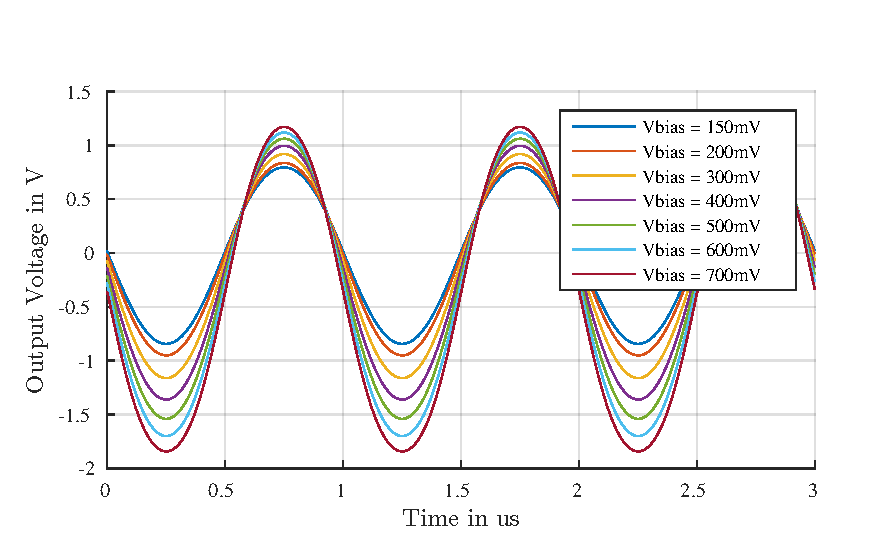
\includegraphics[scale=1]{Figures/Plots/OTA_Sine.pdf}
\caption{OTA Output Voltage for vs time for different Vbias}
\label{fig:OTA_Sine}
\end{figure}

Table\ref{tab:OTA_Sine_Params} shows the variation of different transient parameters with respect to $V_{bias}$. The voltage swing varies from 1.639 to 3.014 which is almost in the ratio of 1:2. HD3 worsens with increase in $V_{bias}$ and on the contrart, improves. Although, it is seen that the HD2 again starts to worsen beyond 600mV of $V_{bias}$.

\begin{table} [H]
\centering
\begin{tabular}{@{}cccccccc@{}}
\toprule
Vbias (mV)					& 150			& 200			& 300			& 400			& 500			& 600			& 700 \\ \midrule
Vout Max (V)			& 0.7949		& 0.8362		& 0.9188		& 0.995		& 1.061		& 1.119		& 1.172 \\
Vout Min (V)			& -0.844		& -0.9505		& -1.162		& -1.361		& -1.54		& -1.7		& -1.842 \\
Vout Swing (V)				& 1.639		& 1.787		& 2.081		& 2.356		& 2.601		& 2.818		& 3.014 \\
HD2 (dBc) 				& -44.83		& -44.28		& -43.86		& -44.74		& -47.97		& -60.86		& -48.75 \\
HD3 (dBc) 				& -52.15		& -49.69		& -46.13		& -43.87		& -42.24		& -40.78		& -39.32 \\
\bottomrule
\end{tabular}
\caption{Transient Parameters of the OTA}
\label{tab:OTA_Sine_Params}
\end{table}

\subsubsection{Square Input}
The test bench in Figure.(f) is used to measure the transient parameters for a square wave input. Slew rate is the rate of change of output voltage. It is also defined as the ratio of bias current to load capacitance.

$V_{DD}$ = 2.5V; $V_{SS}$ = -2.5V; $V_{cm}$ = 1.95V; $V_{bias}$ = 150mV to 700mV;  $V_{pulse} V_1$ = 100mV; $V_2$ = -100mV; $Pulse Width$ = 49.7ns; $Period$ = 100ns; $Rise Time$ = 300ps; $Fall time$ = 300ps; $C_{L}$ = 50fF.

The slew rate, both for the rising edge and the falling edge is tabulated in the Table.\ref{tab:OTA_Slew}.

\begin{table} [H]
\centering
\begin{tabular}{@{}cccccccc@{}}
\toprule
Vbias (mV)					& 150			& 200			& 300			& 400			& 500			& 600			& 700 \\ \midrule
Slew Rate Rising Edge (V/us)			& 386.9		& 407.8		& 452.9		& 501.9 	& 547.6		& 585.4		& 609.3 \\
Slew Rate Falling Edge (V/us)			& -389		& -413.8		& -469.4		& -523.5		& -570.5		& -605.7		& -626.4 \\
\bottomrule
\end{tabular}
\caption{Slew Rate of the OTA}
\label{tab:OTA_Slew}
\end{table}

\section{Summary}